\documentclass[tikz,border=2pt]{standalone}
\usepackage{tikz}
\usetikzlibrary{positioning,arrows.meta}
\begin{document}
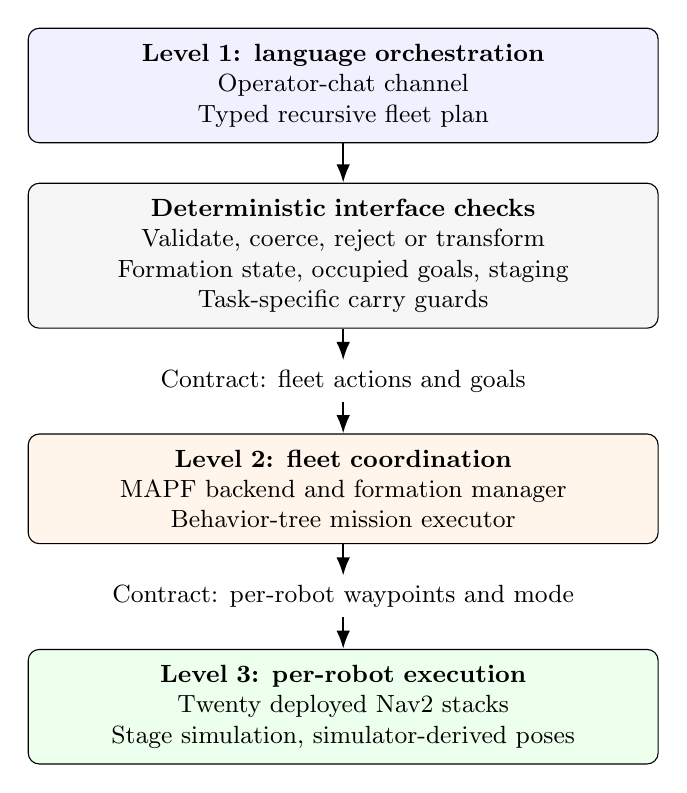
\begin{tikzpicture}[
 n/.style={draw,rounded corners,align=center,text width=76mm,
 inner sep=2mm,font=\fontsize{9.5}{11}\selectfont},
 c/.style={align=center,font=\fontsize{9.5}{11}\selectfont},
 a/.style={-{Latex},thick}]
\node[n,fill=blue!6] (l) {\textbf{Level 1: language orchestration}\\
Operator-chat channel\\
Typed recursive fleet plan};
\node[n,fill=gray!7,below=5mm of l] (g) {\textbf{Deterministic interface checks}\\
Validate, coerce, reject or transform\\
Formation state, occupied goals, staging\\
Task-specific carry guards};
\node[c,below=4mm of g] (c1) {Contract: fleet actions and goals};
\node[n,fill=orange!8,below=4mm of c1] (m) {\textbf{Level 2: fleet coordination}\\
MAPF backend and formation manager\\
Behavior-tree mission executor};
\node[c,below=4mm of m] (c2) {Contract: per-robot waypoints and mode};
\node[n,fill=green!7,below=4mm of c2] (r) {\textbf{Level 3: per-robot execution}\\
Twenty deployed Nav2 stacks\\
Stage simulation, simulator-derived poses};
\draw[a] (l)--(g);
\draw[a] (g)--(c1);
\draw[a] (c1)--(m);
\draw[a] (m)--(c2);
\draw[a] (c2)--(r);
\end{tikzpicture}
\end{document}
